\section{Geração de índices candidatos}
\label{geracao-indices-candidatos}

A geração de índices candidatos envolve analisar as consultas que foram informadas no arquivo de entrada da ferramenta, identificando quais são os campos das tabelas que são incluídos mais frequentemente em condições de filtro, como WHERE e JOIN, bem como em outras cláusulas da consulta que afetam a forma como os dados são recuperados do banco de dados, como GROUP BY e ORDER BY.

O processo de geração dos índices candidatos deve ser otimizado de forma a não sugerir índices que ofereçam ganhos pouco significativos, visando reduzir o tempo de processamento da etapa seguinte - a estimativa de custo das consultas. Com esse objetivo, o MIST foi desenvolvido considerando as recomendações de melhores práticas na criação de índices especificamente para o banco de dados MySQL \cite{MySQL57Ref:Indexes}. Essas recomendações são utilizadas no momento de combinação de colunas para formação dos índices, influenciando na ordem em que as colunas são indexadas, como apresentado na figura \ref{fig:geracao-candidatos}.

\begin{figure}[!ht]
  \centering
  \caption{Processo de geração de índices candidatos.}
  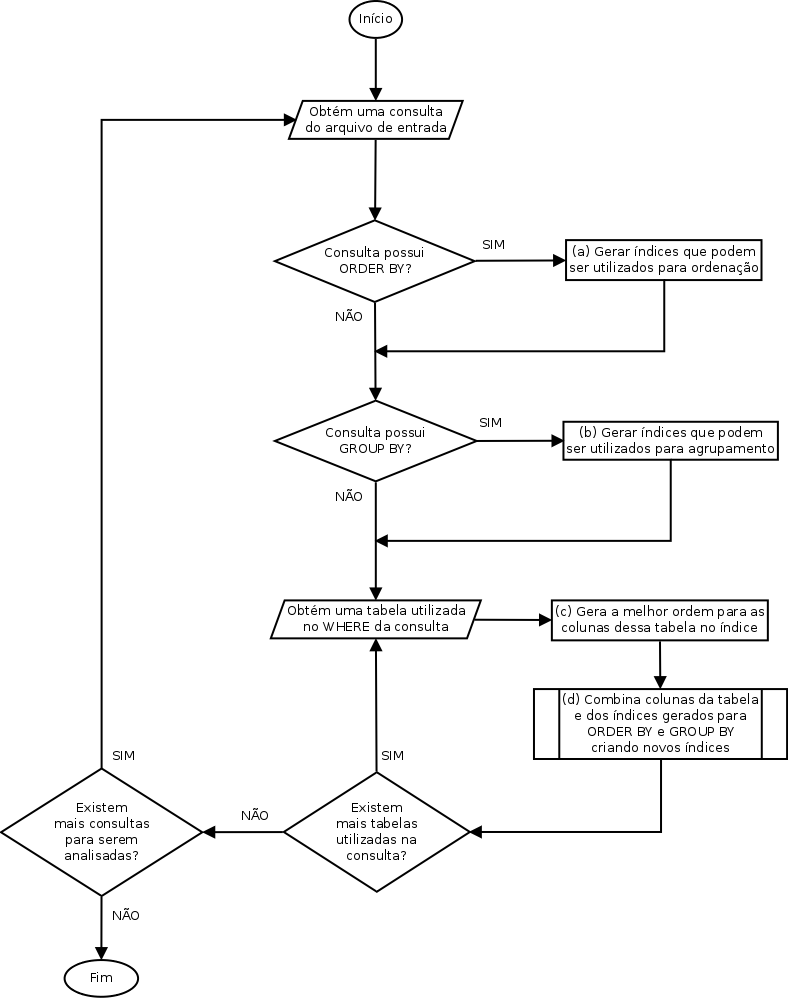
\includegraphics[width=\textwidth]{geracao-candidatos.png}
  \fonte{Elaborado pelo autor.}
  \label{fig:geracao-candidatos}
\end{figure}

Podem ser identificadas nesta figura quatro etapas intermediárias essenciais para a geração dos índices candidatos de forma otimizada, que são executadas para todas as consultas do \textit{workload} analisado. Em (a) são identificadas as colunas incluídas na cláusula ORDER BY da consulta, limitando-se a colunas de uma mesma tabela. Em (b) um processo semelhante é realizado para as colunas da cláusula GROUP BY. A saída dessas duas etapas são os índices mais específicos que podem ser utilizados para ordenação e agrupamento dessa consulta, e são armazenados temporariamente para inclusão em uma etapa posterior.

Após as etapas (a) e (b) serem concluídas, as etapas (c) e (d) são executadas repetidamente para cada tabela diferente incluída na consulta que está sendo analisada. A etapa (c) aplica algumas recomendações e boas práticas para a construção de índices, conforme descrito por \citeonline{Lightstone:2007}. Dessa forma, a implementação do MIST considera uma sequência adequada para escolher as colunas que formarão os índices sugeridos, conforme enumerado a seguir:

\begin{enumerate}
    \item colunas que são utilizadas em comparação de igualdade com valores constantes (parâmetros de comparação informados no SQL) no WHERE ou no JOIN;
    \item colunas que são utilizadas em comparação de igualdade com outras colunas no WHERE ou no JOIN;
    \item colunas utilizadas no WHERE em condições de busca por intervalo de valores;
    \item colunas utilizadas em comparação com uma lista de valores constantes (por exemplo, utilizando a construção IN do SQL);
    \item colunas utilizadas com o operador LIKE;
\end{enumerate}

Além do tipo de comparação realizado entre as colunas nas condições de WHERE e JOIN, outros fatores também são determinantes na decisão das colunas que serão adicionadas ao índice, a saber:

\begin{itemize}
    \item para uma consulta que possui agrupamento e ordenação, só é possível utilizar índices para a operação de agrupamento. Assim, as colunas que estão presentes apenas na cláusula ORDER BY da consulta não são consideradas para o índice;
    \item índices candidatos formados por colunas que correspondem a um prefixo da chave primária da tabela são desconsiderados, uma vez que esses seriam preteridos em favor do índice primário durante a otimização da consulta;
\end{itemize}

Ainda, o MIST não considera colunas do tipo BLOB ou TEXT para serem utilizadas em índices. Isto se deve ao fato de que o MySQL não oferece suporte à indexação da coluna completa para estes tipos de dados, sendo necessário sempre informar o tamanho de um prefixo para ser indexado nessas colunas. Visando simplificar o desenvolvimento, a identificação do tamanho do prefixo ideal para estas colunas não foi implementada no MIST, impossibilitando, desta forma, que tais colunas sejam incluídas nos índices gerados.

A etapa (d) apresentada no diagrama da figura \ref{fig:geracao-candidatos} é responsável por reunir os resultados das três etapas anteriores e gerar os índices candidatos.

A interface do MIST que exibe os índices candidatos gerados é exibida na figura \ref{fig:mist-candidatos-gerados}. Os índices são exibidos no formato de uma tabela, onde cada linha corresponde a um índice candidato gerado. As duas primeiras colunas contém a definição do índice, enquanto a terceira, "Consultas Afetadas", apresenta a quantidade de consultas que serão impactadas pelo índice.


\begin{figure}[!ht]
  \centering
  \caption{Interface do MIST exibindo índices candidatos gerados.}
  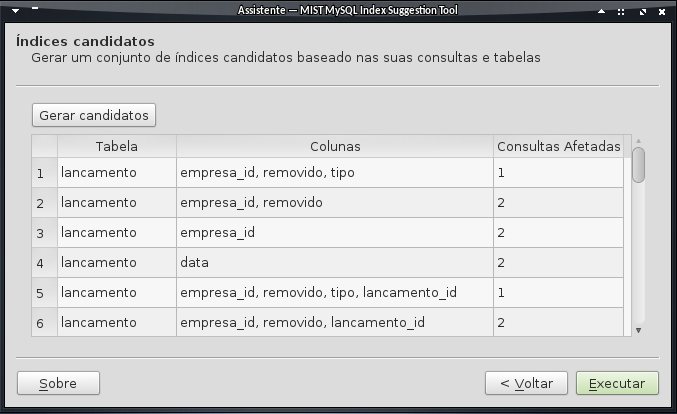
\includegraphics[width=\textwidth]{mist-indices-candidatos.png}
  \fonte{Elaborado pelo autor.}
  \label{fig:mist-candidatos-gerados}
\end{figure}
